%%MaD.tex - Notes taken for Materials and Devices Lecture
%%Author: Andy Goetz
%%Date Modified: 10-7-09
%%License: Ask me before reproducing/modifying, etc.


\documentclass{article}

%Make sure you have the file ShumanNote.scy in the same directory as
%this one. It has contains the style sheet for ECE111, and is needed
%to standardize the layout of LateX documents created for the class.
\usepackage{ShumanNotes} 
\usepackage{multirow}
\usepackage{tikz}
\usepackage{program}
\usepackage{listings}
\pdfpagewidth 8.5in 
\pdfpageheight 11in

%This package is used to line up pictures 
\usepackage{graphicx}
\usepackage{fancyvrb}
\usepackage{listings}
%allows cursive font
%\usepackage{amsmath}

%allows hyperlinks 
%\usepackage{hyperref}

\newcommand{\HRule}{\rule{\linewidth}{0.5mm}} 

\lhead{T-16 User Manual}

\begin{document}

%% These commands allow me to use cursive letter for things such as
%% length.  Note that on ubuntu linux, this required installation of
%% the package 'texlive-fonts-extra'. 
%% Taken from
%% http://www.latex-community.org/forum/viewtopic.php?f=5&t=1404&start=0
\newenvironment{frcseries}{\fontfamily{frc}\selectfont}{}
\newcommand{\textfrc}[1]{{\frcseries#1}}
\newcommand{\mathfrc}[1]{\text{\textfrc{#1}}}

\begin{titlepage}
 
\begin{center}
 
 
\textsc{\LARGE Womprat T-16 Audio Synthesizer}\\[1.5cm]
 
\textsc{\Large Portland State University}\\[0.5cm]
 
 
% Title
\HRule \\[0.4cm]
{ \huge \bfseries User Manual}\\[0.4cm]

 
\HRule \\[1.5cm]


\includegraphics[width=3in]{womprat-bitmap.png}
\vfill
 
% Author and supervisor
\begin{minipage}{0.4\textwidth}
\begin{center} \large
Andy \textsc{Goetz}, Bradon \textsc{Kanyid}, Jackson \textsc{Pugh}, and Kevin \textsc{Riedl}\\
\end{center}
\end{minipage}

 
 
\end{center}

{ \textit{} }\\[4.0cm]
\begin{center}
% Bottom of the page
{\large \today}

\end{center} 
\end{titlepage}

\newpage

\textbf{\large Version}
\vspace{.1in}

\begin{tabular}{|p{1in}|p{4in}|p{1in}|}
\hline
\multicolumn{3}{|l|}{\textbf{Document Review}} \\ 
\hline
\textbf{Version}& \textbf{Comments} & \textbf{Date} \\ 
\hline
\textbf{1.0} & Initial release. & 11/24/12 \\
\hline
\end{tabular}

\newpage
 
\centerimage{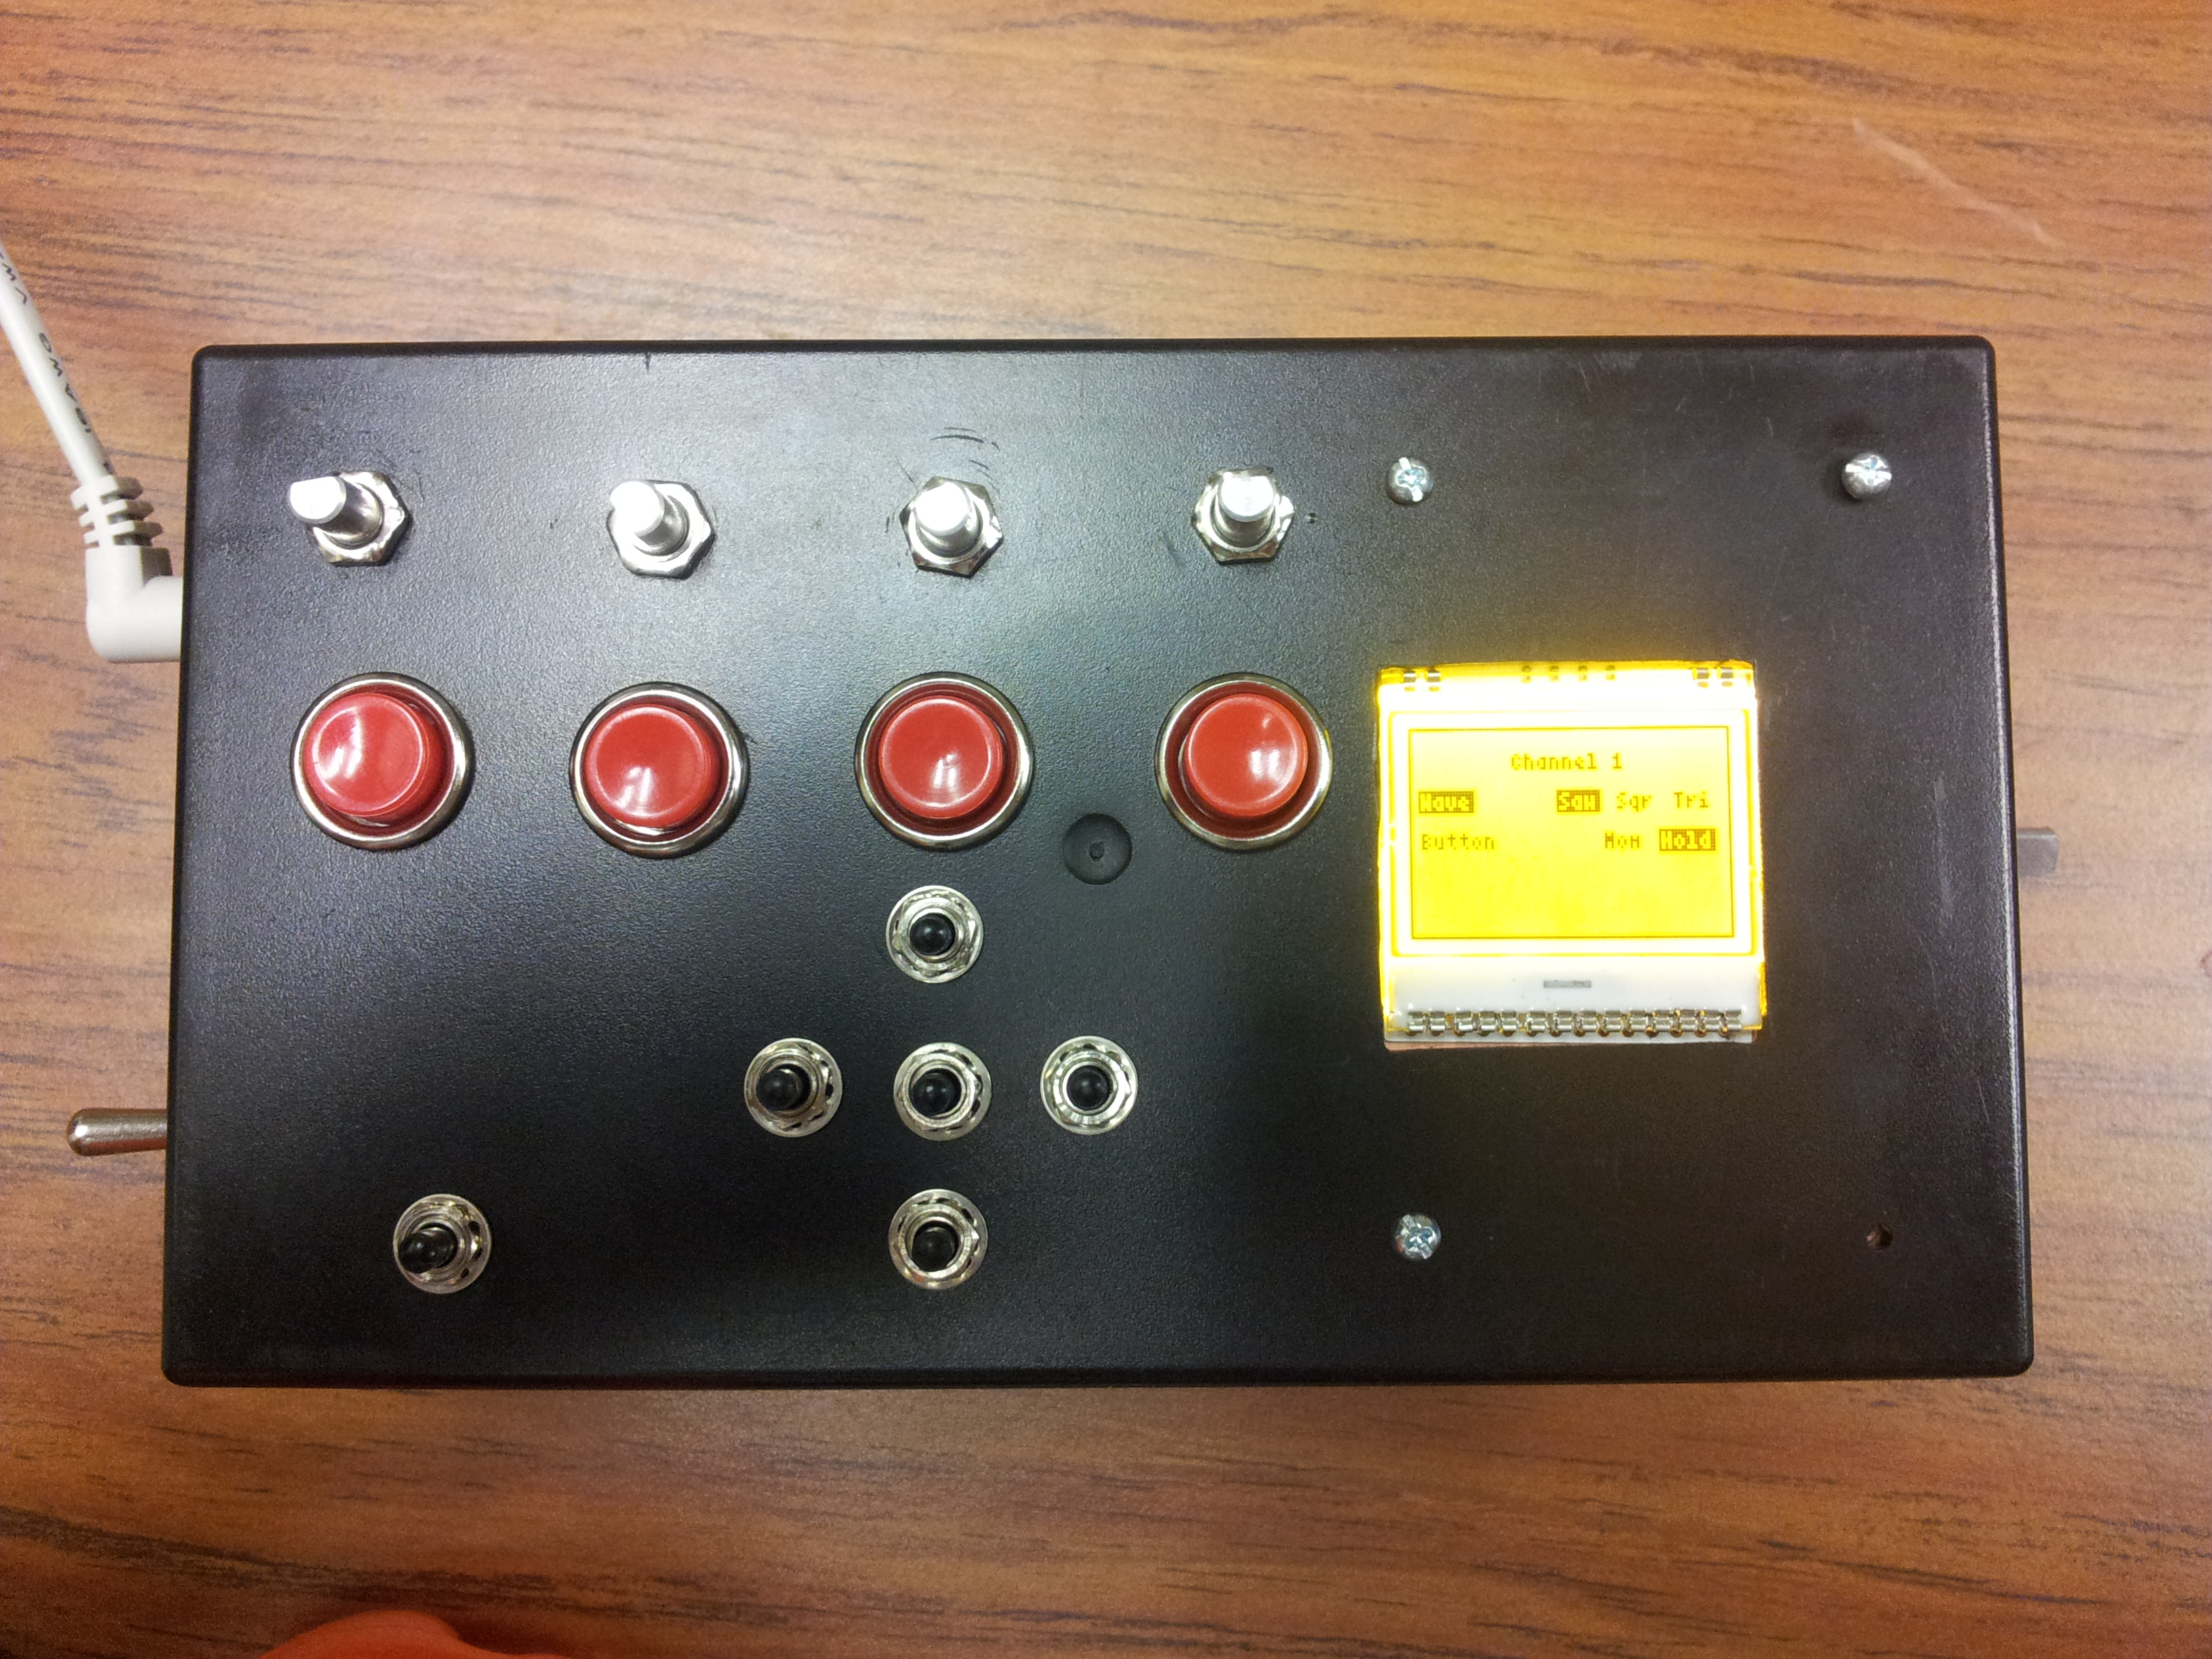
\includegraphics[width=5in]{unannotated.png}}{T-16 Audio Synthesizer}{synth}

\section{Overview}




\newpage
\setcounter{tocdepth}{2}
\tableofcontents

\newpage

\section{User Interface}

\centerimage{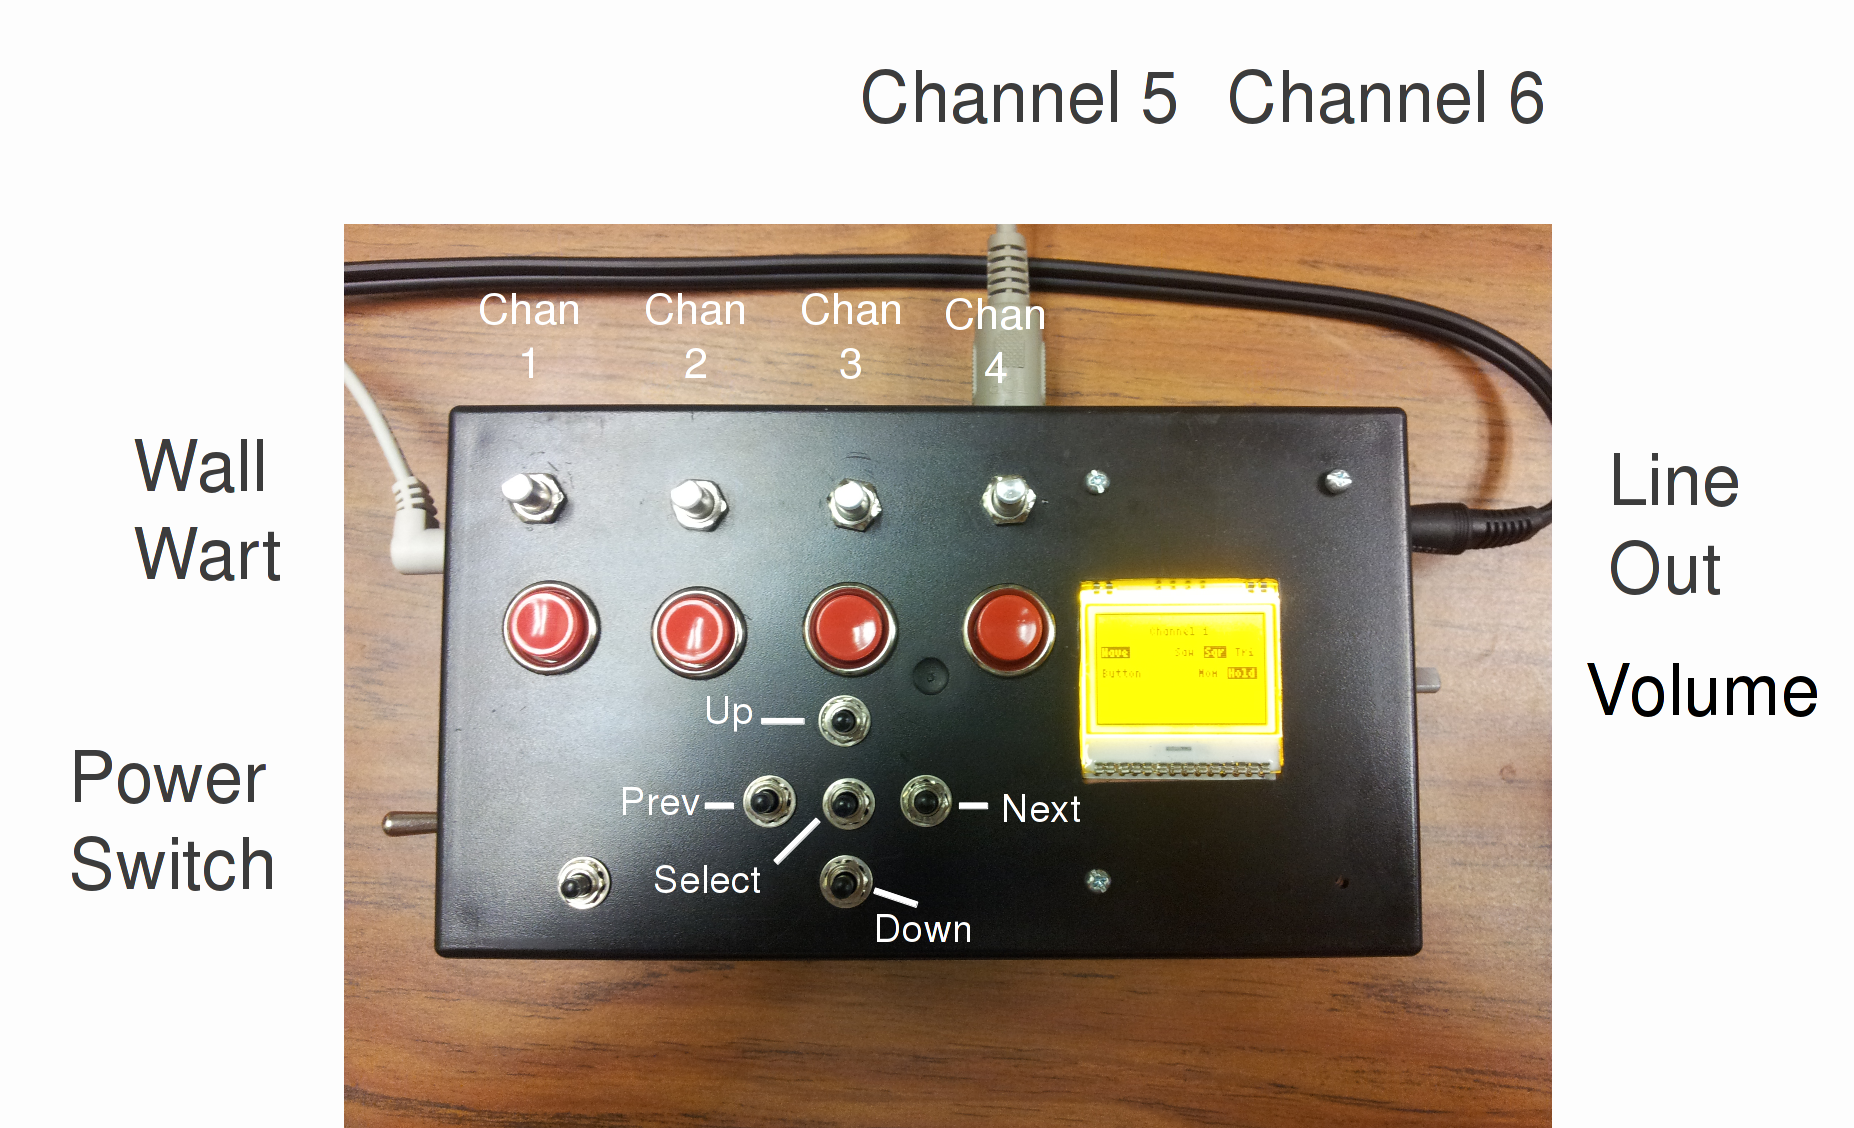
\includegraphics[width=5in]{womprat-annotated.png}}{T-16 User Interface}{annotated}

\subsection{LCD}

\centerimage{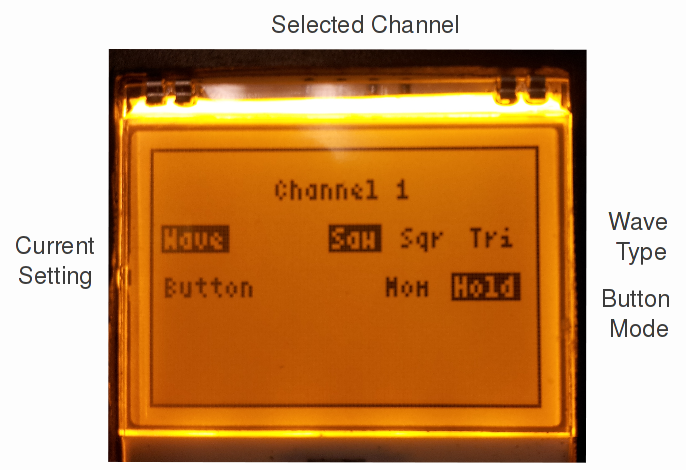
\includegraphics[width=5in]{LCD-annotated.png}}{LCD}{lcd}

\section{Input Power}

\section{External Interface}


\end{document}
